\documentclass[border={5pt 5pt 5pt 5pt}, preview]{standalone}

% Math & Symbol packages
\usepackage{amsmath}
\usepackage{amssymb}

% Graphics & Float packages
\usepackage{float}
\usepackage{graphicx}
\usepackage{subfigure}
\usepackage{tikz}
\usetikzlibrary{patterns, arrows.meta, calc}
\usepackage{pgfplots}
\pgfplotsset{compat=newest}

% Colors
\usepackage{xcolor}
\definecolor{HMSRed}{HTML}{C5112E}  % [197, 17, 46]
\definecolor{MGHBlue}{HTML}{008BB0} % [0, 139, 176]
\definecolor{MGHGrey}{HTML}{626365} % [98, 99, 101]

\begin{document}

\begin{figure}[htp]
\centering
    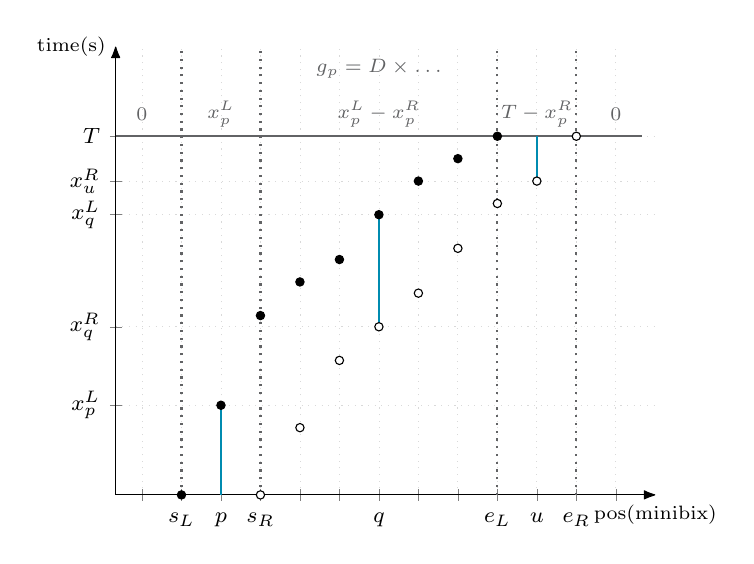
\begin{tikzpicture}
        \pgfplotsset{holdot/.style={color=black,only marks,mark=*,mark size=1.5pt}}
        \pgfplotsset{soldot/.style={color=white,only marks,mark=*,mark size=1.5pt}}
        \begin{axis}[
            xmin=0.5, xmax=10.75,
            ymin=0, ymax=10,
            grid = both,
            grid style = dotted,
            grid style = {line width=.1pt, draw=gray!10},
            major grid style = {line width=.3pt,draw=gray!30},
            axis lines = middle,
            enlargelimits = {abs=0.0},
            axis line style = {-Latex[round]},
            ticklabel style = {font=\footnotesize},
            xticklabel style = {text height=1ex},
            xticklabels = {,$s_L$,$p$,$s_R$, , , $q$, , ,$e_L$,$u$,$e_R$},
            xtick = {1,1.75,2.5,3.25,4,4.75,5.5,6.25,7,7.75,8.5,9.25,10},
            yticklabels = {$0$,$x_p^L$, $x_q^R$, $x_q^L$, $x_u^R$, $T$},
            ytick = {0,2,3.75,6.25,7,8},
            xlabel style = {at={(ticklabel* cs:1)},anchor=north},
            ylabel style = {at={(ticklabel* cs:1)},anchor=east},
            xlabel = {\scriptsize{pos(minibix)}},
            ylabel = {\scriptsize{time(s)}},
        ]

            % Dashed line at height T
            \draw[color=MGHGrey, thick] (0.5,8) -- (10.5,8);

            % Leaf trajectories
            \addplot[fill=black, color=black, only marks, mark=*, mark size = 1.5pt]
                coordinates{(1.75,0.0)(2.5,2.0)(3.25,4.0)(4.0,4.75)(4.75,5.25)(5.5,6.25)(6.25,7.0)(7.0,7.5)(7.75,8.0)};
            \addplot[fill=white, only marks, mark=*, mark size = 1.5pt]
                coordinates{(3.25,0.0)(4.0,1.5)(4.75,3.0)(5.5,3.75)(6.25,4.50)(7.0,5.50)(7.75,6.5)(8.5,7.0)(9.25,8.0)};

            % Different sectors
            \draw[color=MGHGrey, thick, dotted] (1.75,0) -- (1.75,10);
            \draw[color=MGHGrey, thick, dotted] (3.25,0) -- (3.25,10);
            \draw[color=MGHGrey, thick, dotted] (7.75,0) -- (7.75,10);
            \draw[color=MGHGrey, thick, dotted] (9.25,0) -- (9.25,10);

            % Exposure times
            \draw[color=MGHBlue, thick] (2.5,0) -- (2.5,2);
            \draw[color=MGHBlue, thick] (5.5,3.75) -- (5.5,6.25);
            \draw[color=MGHBlue, thick] (8.5,7) -- (8.5,8);

            % Exposure
            \node[color=MGHGrey] at (5.5 ,9.5) {\scriptsize{$g_p = D \times \hdots$}};
            \node[color=MGHGrey] at (1.0 ,8.5) {\scriptsize{$0$}};
            \node[color=MGHGrey] at (2.5 ,8.5) {\scriptsize{$x_p^L$}};
            \node[color=MGHGrey] at (5.5 ,8.5) {\scriptsize{$x_p^L-x_p^R$}};
            \node[color=MGHGrey] at (8.5 ,8.5) {\scriptsize{$T-x_p^R$}};
            \node[color=MGHGrey] at (10.0,8.5) {\scriptsize{$0$}};
        \end{axis}
    \end{tikzpicture}
    
\caption[Illustration of the total minibixel exposure $g_p$, $p \in \mathcal{P}\backslash\{P\}$]{
    Illustration of the total minibixel exposure $g_p$, $p \in \mathcal{P}\backslash\{P\}$.
    The total minibixel exposure is calculated using four cases, see \eqref{eq:LRG}.
    Closed and open dots indicate the trajectory of the left and right leaf, respectively.
    }
\label{fig: exp cases}
\end{figure}

\end{document} 